\chapter{Detecting Twitter events}


\section{Introduction}
Twitter has been used to detect or predict a large variety of events,
from flood prevention \cite{de2017towards} to stock market movements
\cite{pagolu2016sentiment}. However, the specificity of social network data (short texts, use of
slang, abbreviations, hashtags, images and videos, very
high volume of data) makes all "general" detection tasks
(without specification
of the type of topic)
very difficult on tweet datasets.

Many works on event detection are actually
focused on burst detection (detecting topics such as
natural disasters, attacks, etc., that cause an unusual
volume of tweets), and do not attempt to assess the
relative size of events. We seek to detect \textit{all} events, both
those that generate a high volume of tweets and those that
are little discussed, and to group together \textit{all} tweets
related to the same event. With this definition in mind, the
topic detection and tracking task is conceptually similar to 
clustering. Given the size of our tweet collection, 
the chosen clustering method has to be extremely time-efficient.

Apart from the choice of the event detection algorithm, 
we also have to consider the type of tweet representation: 
should we only use the text of the tweets, or should we consider 
the tweet as a multimodal document, composed of text and/or images, videos, hashtags?

In the field of language processing, recent works
have made it possible to reach performance close to human capacity
in several tasks, 
particularly with regard to the evaluation of the semantic similarity 
between two sentences\footnote{See the results on the GLUE benchmark: \url{https://gluebenchmark.com/leaderboard}}. However, these advances, 
based on the training of neural networks on very large corpora of texts,
may not always be suited to our task. Indeed, despite rapid progress 
in recent years in the adaptability of
language processing (the GLUE benchmark \cite{wang2018glue} consists of
9 different tasks, and the models are evaluated according to their average performance on
all these tasks), it remains difficult to adapt these models to new tasks. 
Any transformation of the initial task requires fine-tuning a neural network 
on (at least) a few thousand sentences, which
involves hours of manual annotation to create a suitable dataset. 
In our work we focus on short-text topic similarity (evaluate if two sentences / short texts
address the same subject), which in some cases differs from semantic similarity
(evaluate whether two sentences mean the same thing) evaluated in GLUE, and we don't 
have a corresponding training dataset. Besides, even on a strictly identical
task, the performances announced in the litterature are perfectly reproducible 
only on English language corpora. 

Finally, most of these models are designed to be used as input to
end-to-end systems. For example, to calculate a similarity score between sentences
with BERT \cite{devlin2018bert}, it is necessary to treat each couple of sentences instead of each sentence. Using the example proposed in \cite{reimers_2019_sentence}, to find the two most similar sentences in a corpus of $n = 10,000$ sentences, the number of treatments to be performed is $n\frac{(n - 1)}{2} = 49,995,000$ operations, which represents approximately 65 hours of processing with BERT on a V100 GPU.
These architectures do not apply well to information retrieval systems that involve comparing
hundreds of thousands of sentences. For clustering or information retrieval tasks, 
it is more efficient to represent each sentence in a vector space where similar sentences
 are close (so-called \textit{embeddings}), and then apply conventional distance measurements 
 (cosine, euclidean distance, etc.).
 
 \begin{figure*}
  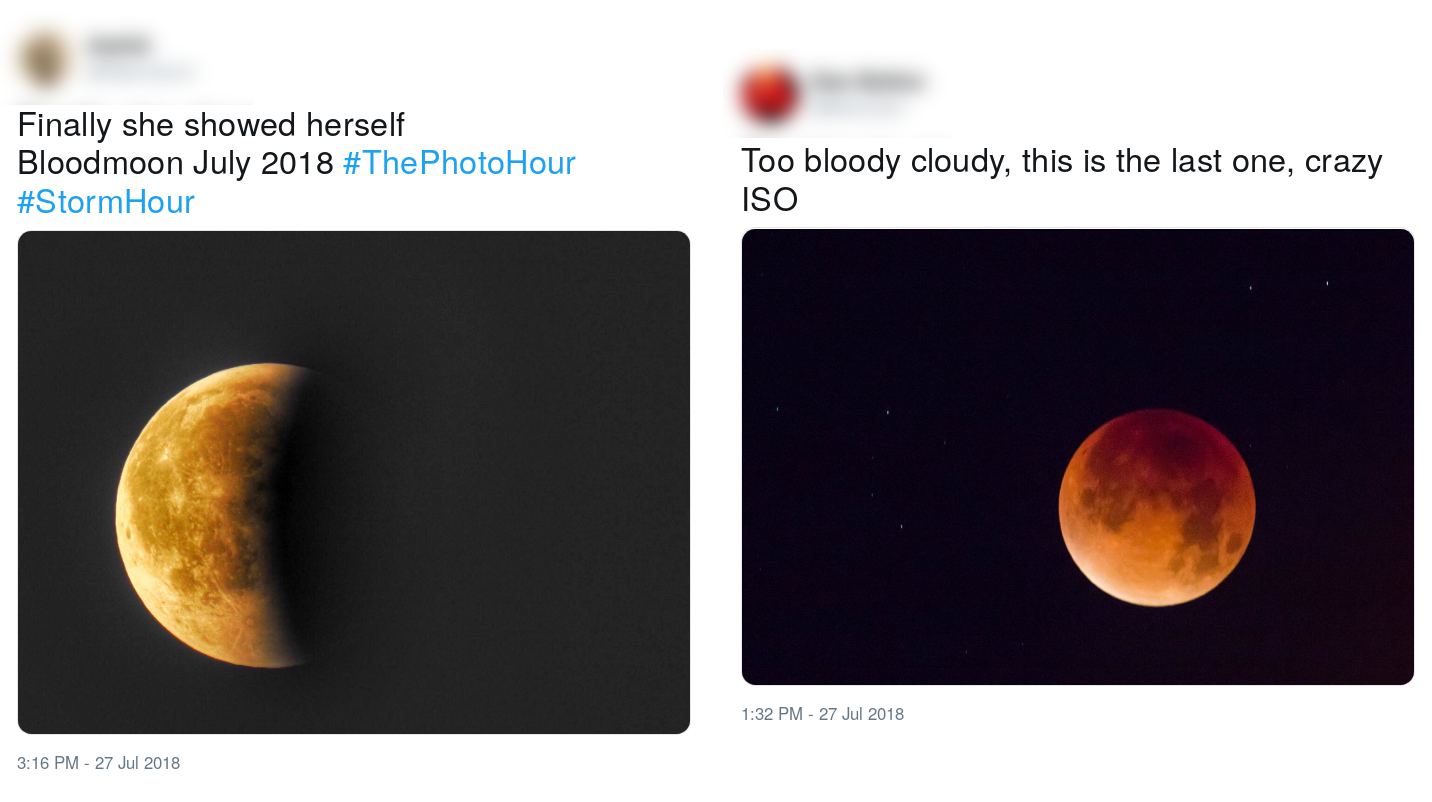
\includegraphics[width=\textwidth]{figures/Moon_horizontal.png}
    \caption{Example of a topic (the July 2018 lunar eclipse) where multimedia contents provide a critical information for topic detection}
    \label{fig:moon}
\end{figure*}
 
 Regarding images, recent progress in the field of visual content description due to deep neural networks provides new ways of representing social media documents by including rich visual features. There are cases where image provides decisive information for event detection (see Fig. \ref{fig:moon}). However, dealing with image tweets often requires a contextual knowledge external to the document. Without this knowledge, image can become a source of error for event detection algorithms compared to text alone.
 
We deepen these questions throughout the chapter, starting with a state of the art, then presenting different tested algorithms. Finally, we present the results of our experiments, first on text, then using multimodal approaches.


\section{State of the art}

		
		\subsection{Twitter event detection approaches}
		We divide the event detection methods into three types of approaches: term-weighting-based approaches, topic modeling, and clustering. This is also the classification used in the survey on real-time event detection by \citet{hasan_survey_2018}. The last approach, clustering, is dealt with in more detail in this state of the art, as it is the one we chose to implement for our own event detection tool.
		
		\subsubsection{Term-weighting-based approaches}
		These approaches rely on tracking the terms likely to be linked to an event (often due to a high frequency of some terms during a given time window). They usually return a list of the top $k$ trending events on Twitter, which does not meet our objective of detecting events in an exhaustive manner.
		
		The event detection system TwitterMonitor \citep{mathioudakis_twittermonitor:_2010} detects bursty keywords in the Twitter stream by comparing their term frequencies in previous periods to current term frequency. Bursty keywords are then grouped together in ``trends" depending on their co-occurrences in recent tweets. 
		
		EnBlogue \citep{alvanaki_see_2012} measures the correlation of hashtags pairs within a given time window. Emergent topics are then detected among the pairs with the highest shift in their correlation. EnBlogue produces an overall scoring of the topics depending on the shift in correlation and on the total popularity of each topic. This score is smoothed in order to give a higher rank to new topics. 
		
		MABED \citep{guille_event_2015} does not only uses the textual content of the tweets: the frequency at which users interact with each other using ``mentions" (i.e. the name of another Twitter account preceded by ``@") is also taken into account to detect events. The system models the number of tweets that contain word $t$ and at least one mention during a given time-window as a binomial distribution. It detects positive anomalies if the creation of mentions associated to word $t$ is strictly greater than the expectation of the model. The magnitude of impact of an event on a time interval I is computed by integrating the anomaly function on the interval I. For each word associated with a mention, the system finds the interval I that maximizes its magnitude of impact. After other steps of event description and duplicates removal, the events with the highest impact are returned.
		
		The Twitter Live Detection Framework (TLDF) \citep{gaglio_framework_2016} modifies the Soft Frequent Pattern Mining (SFPM) algorithm \citep{petkos_soft_2014} to adapt to the dynamic nature of tweets. The authors use the relevance score of term $t$ proposed for SFPM: the ratio of the likelihood of appearance of the term in the current time-window and in a reference set of tweets. This relevance score is combined with a parameter boosting the score of named entities and multiplied by the $\mbox{tf-idf}$ of term $t$. Moreover, the size of the detection time-window is not fixed, but is controlled by a sigmoid function depending on the volume of emitted tweets at a given moment.
	
	\subsubsection{Topic models} Topic models are widely used techniques in the natural language processing field to discover the topical structure from a corpus of textual documents (news articles, scientific papers, tweets, etc.). Latent Dirichlet Allocation (LDA) is the most common one \citep{blei_latent_2003}. In this model, each document is considered as a mixture of different topics drawn from a topic distribution. 
	
	In our case, LDA has several drawbacks: 1. it assumes that a document is a mixture of several topics, which is very rare in short texts like tweets, 2.the model does not take into account the fact that topics change over time, 3. the number of topics has to be known in advance. There is however a vast literature working on strategies to overcome these limitations. The recent survey by \citet{likhitha975detailed} summarizes the topic modeling techniques used to find topics within short text documents.
	
	\begin{enumerate}
	 \item To adapt LDA to short texts, several approaches have been proposed in past works: one of them, known as Dirichlet Multinomial Mixture (DMM) model is to restrict the document-topic distribution, such that each tweet is assumed to be generated from a single topic \citep{yin_dirichlet_2014}. \citet{li_enhancing_2017} propose to extend the DMM model by allowing short texts to be generated by one or more topics, where the topic number is reduced (from 1 to 3) and drawn from a Poisson distribution.
	 \item \citet{blei_dynamic_2006} have addressed the issue of topics evolving over time; however they assume that the number of topics remains the same over periods, whereas in a stream of tweets, topics can emerge and disappear at each new period.
 	 \item Regarding the number of topics, some methods exist to estimate the optimal parameter $k$  \citep{brunet_metagenes_2004,arun_finding_2010,greene_how_2014}. However these methods rely on re-generating topic models for each candidate $k \in [k_{min}, k_{max}]$. This can be achieved for a small number of topics ($k_{max} < 100$), but testing each $k$ in a range $[2100, 10500]$ (between 100 and 500 events a day in our corpus of 21 days) is not an option. For this reason, we have favoured a clustering approach rather than topic modeling techniques.
	\end{enumerate}


	\subsubsection{Dynamic clustering \label{Subsubsec: incremental clustering}} Dynamic clustering approaches do not require a fixed number of clusters. These methods are well fitted for discovering clusters of textual documents dynamically as new documents are added to the collection. For this type of clustering, algorithms are often used that take into account both the thematic similarity of the documents and their temporal proximity, in order to avoid grouping in the same cluster tweets sent at very distant times. This type of approaches generally use the state of the art First Story Detection (FSD) \citep{allan_introduction_2002} algorithm as reference method. In this method (see Algorithm 1), documents are represented using tf-idf (see Section \label{Text embeddings} for a presentation of tf-idf encoding), their similarity is computed using cosine similarity, and each new document joins the cluster of its nearest neighbor in the collection. If the distance to the nearest neighbor is higher than a pre-defined threshold $t$ a new cluster is created, that contains the new document. Regularly, the oldest documents are dropped from the collection. This insures that each new document is only compared to the most recent documents. 

%%%%%%%%%%%%%%%%%%%%%%%%%%%%%%%%%%%%%%%%%%%%%%%%%%%%%%%%%%%%
\label{FSD}
\begin{algorithm}
\caption{``First Story Detection"}
\begin{algorithmic}[1]
\REQUIRE threshold $t$, window size $w$, corpus $C$ of documents in chronological order
\ENSURE thread ids for each document
\STATE $T \leftarrow \left[ \right] ; i \leftarrow 0 $
\WHILE{document $d$ in $C$}
\IF{$T$ is empty}
\STATE $thread\_id(d) \leftarrow i$
\STATE $i \leftarrow i+1$
\ELSE
\STATE $d_{nearest} \leftarrow $ nearest neighbor of $d$ in $T$
\IF{$cosine(d, d_{nearest}) < t$}
\STATE $thread\_id(d) \leftarrow thread\_id(d_{nearest})$
\ELSE
\STATE $thread\_id(d) \leftarrow i$
\STATE $i \leftarrow i+1$
\ENDIF
\ENDIF
\IF{$|T| \geq w$}
\STATE remove first document from $T$
\ENDIF
\STATE add $d$ to $T$
\ENDWHILE
\end{algorithmic}
\end{algorithm}
%%%%%%%%%%%%%%%%%%%%%%%%%%%%%%%%%%%%%%%%%%%%%%%%%%%%%%%%%%%%



Existing works on tweet incremental clustering have adapted this reference method initially developed for streams of news (such as RSS streams) to process much higher volumes of documents, and very short texts. Indeed the maximum size of a tweet is 280 characters (140 characters before 2018). Changes in that baseline method are done either in the type of text representation, or in the clustering algorithm itself. A step of noise filtering is also frequently added before the clustering step, to distinguish event from non-event tweets (according to \citet{liu_reuters_2016}, the proportion of event tweets in well established corpora such as the one by \citet{mcminn_building_2013} is less than 0.2\%). This section explores the variations introduced in the clustering algorithm.


In TwitterStand, \citet{sankaranarayanan_twitterstand:_2009} first perform a filtering step, that classify tweets as either ``junk" or ``news" using a naive Bayes classifier. Then, their online clustering algorithm associates a vector to each cluster, which is composed from the contained tweets' terms weighted with tf-idf. Each new tweet is represented using tf-idf and compared to the clusters' vectors using a modified cosine distance that accounts for the temporal dimension of clusters. The distance formula is 
$$
\dot{\delta}(t,c) = \delta(t,c)\times e^{\frac{-(T_t-T_c)^2}{2\sigma^2}}
$$

where $\delta(t,c)$ is the cosine distance between tweet $t$ and cluster $c$, $T_t$ is tweet $t$'s publication time and $T_c$ is cluster $c$'s mean publication time. The distance is only computed for clusters with a mean publication time $T_c$ more recent than 3 days, and that have a word in common with $t$. If $\dot{\delta}(t,c^*) \leqslant \epsilon$ (where $c^*$ is the nearest cluster to $t$), the tweet $t$ is added to the cluster $c^*$. Else, a new cluster is created. To speed up the search for the nearest cluster, an inverted index of the cluster's words is maintained: for each word $w$, the inverted index stores pointers to the clusters that contain $w$. The clustering algorithm in TwitterStand is adapted to the noisy nature of tweets by maintaining a list of reputable sources. A cluster is dropped from the list of active clusters if none of the first $k$ tweets are from a reputable source. The system also deals with fragmentation (the fact that several clusters about the same topic are created) by removing duplicate clusters. If a cluster $c'$  is identified as the duplicate of an older cluster $c$, $c'$ is marked as ``slave" of the cluster $c$, and $c$ as ``master" of $c'$. Any tweet that should be added to $c'$ is now added to $c$.

\citet{petrovic_streaming_2010} speed up the standard FSD algorithm by replacing the nearest neighbor search by an approximate nearest neighbor search using Locality Sensitive Hashing. Instead of searching for the nearest neighbor in the set of all documents, the search is done among a small set $S$ of potential nearest neighbors. The set $S$ is the set of documents that have the same hash as current document $x$:
$$
S(x) = \{y: h_{ij}(y) = h_{ij}(x), \exists i \in [1 \ldots L], \forall j \in [1 \ldots k]\}
$$
where $L$ is the number of hash tables, and $k$ the number of hyperplanes in each hash table. The hash functions $h_{ij}$ are defined as:
$$
h_{ij}(x) = sgn(u_{ij}^Tx)
$$
the sign of the scalar product of random vector $u_{ij}$ and $x$. To reduce the risk of failing to find the nearest neighbor (if the nearest neighbor $y$ does not collide with $x$ in the set $S(x)$), if no nearest neighbor is found, the system starts a search of exact nearest neighbor through an inverted index containing only most recent documents. To limit the growth of the sets $S$ (also called buckets), the number of documents in a single bucket is limited to a constant parameter. The oldest documents in the bucket are then removed. 

The system proposed by \citet{petrovic_streaming_2010} has later been improved by the same authors \citep{petrovic_using_2012} using public synonym and paraphrase corpora in order to expand the words of the tweets with all their potential synonyms. This approach is a way to compensate for the scarcity of information contained in tweets and to increase the chances of finding a potential neighbor even if there is no tweet containing the same words in the collection.

\citet{becker_beyond_2011} use the same clustering algorithm as \citet{sankaranarayanan_twitterstand:_2009}, with each new tweet being represented as a tf-idf vector and compared using cosine similarity to the centroid of each cluster (the centroid is the mean weight of all terms in all tweets contained in the cluster). The specificity of their approach lies in the step following the clustering: instead of processing to a noise/event classification at the tweet level, the classification step takes place at the cluster level. They use a wide range of features in order to run a classification algorithm able to distinguish event clusters from noise clusters. The considered features are temporal features (taking into account the frequency of emission of the tweets in the cluster), social features (percentage of messages being retweets, replies, or mentions), topical features (based on the assumption that event clusters have a smaller diversity of topics), and Twitter-Centric features (hashtag usage, presence of multi-word hashtags).

\citet{mcminn_real_2015} base their event-detection approach on Part Of Speech (POS) Tagging and Named Entity Recognition (NER). Their first step is to extract named entities (persons, locations and organizations) and lemmatized nouns and verbs from each tweets. They then proceed to an aggressive filtering step (95\% of the tweets are removed): the system removes retweets, tweets with no named entities, and tweets containing terms associated with noise (``follow", ``watch", etc.). Then two steps are conducted in parallel: a clustering and a burst detection step. The clustering is based on an inverted index of all named entities: for each new tweet, the tweets containing the same named entities are retrieved from the index. The nearest neighbor is searched among these tweets using tf-idf representation, cosine similarity and a similarity threshold. If a nearest neighbor is found and does not already belong to a cluster, a new cluster is created containing the two tweets. In parallel, the bust detection module looks for bursts in the frequency of the detected entities. Once a burst has been detected, the clusters associated with the given entity are associated to it if the average timestamp of the tweets in the cluster is after the initial burst. The clusters associated to one burst form an event. If an entity associated to another event is mentioned in more than 50\% of the event's tweets, the two events are merged.

With Reuters Tracer, \citet{liu_reuters_2016} propose an event detection system that is also largely based on POS tagging and NER. This system combines a tweet level noise filtering and a cluster level noise filtering. Are considered as ``noise" all tweets and all clusters of tweets that are not linked to an event (in the sense of \citet{mcminn_building_2013}). The clustering algorithm itself is quite different from the standard FSD algorithm. New tweets are added to clusters based on three criteria: (1) Retweets of the same tweets are all added to the same cluster. (2) Tweets containing the same url are all added to the same cluster. (3) Finally, a similarity metric with the existing clusters is computed as follows:
$$
S_i = aN_e + bN_n + cN_v + dN_h
$$
where $N_e,N_n,N_v,N_h$ are the numbers of matching Named Entities, nouns, verbs and hashtags between the tweet and the cluster, and $a, b, c, d$ are learned parameters. Liu and al. explain that their system is primarily based on named entities (``An event is usually defined by \textit{who}, \textit{where} and \textit{what}" according to \citet{mcminn_building_2013}), and that there is no need for high dimensional tf-idf vectors to compute a good similarity function. The obtained clusters, called ``unit clusters" are progressively merged into bigger clusters using the same steps (merging based on retweets, urls, then similarity metric) as the unit clustering step. However, the used $a, b, c, d$ parameters are different.

\citet{hasan_twitternews_2016} use the technique of First Story Detection with LSH developed by \citet{petrovic_streaming_2010}. However, they observe that the $k$ independent random vectors in a single hash table need to be updated every time the size of the input tf-idf vectors increases (which happens at a high rate in Twitter data since the vocabulary evolves faster than in traditional news). To alleviate this problem, they propose a technique using random indexing \citep{sahlgren_introduction_2005}. Random indexing  aims at representing terms with fixed-size vectors. Each term $t$ is associated with two vectors: an index vector and a context vector. The index vector is a random vector. The context vector has the same size as the index vector and it is initialized with zeroes. When a co-occurrence of the term $t$ with another term $t'$ is observed, the context vector of $t$ is updated by adding the index vector of $t'$. A tweet can then be represented as an average of the vectors of each term in the tweet. This tweet representation is then used to perform the LSH approximate neighbors search of the tweet $d$. However, once the set $S$ of all documents that collide with $d$ in a hash table is computed, the exact nearest neighbor search is done using cosine similarity on tf-idf vectors, rather than random indexing vectors. \citet{hasan_twitternews_2016} use this method as a first algorithm in order to detect ``non unique" tweets, that are then clustered using a second algorithm close to the one by \citet{sankaranarayanan_twitterstand:_2009}: this time, the similarity to the clusters' centroids is computed. Hasan et al. explain the use of this two-steps clustering method by the necessity to restrain the number of ``one tweet clusters". A defragmentation step is finally done in order to merge similar clusters.


In these works, tweets are represented in the form of tf-idf vectors in the vast majority of cases \citep{sankaranarayanan_twitterstand:_2009, petrovic_streaming_2010, becker_automatic_2011, hasan_twitternews_2016}. \citet{repp_extracting_2018} test different types of representation of tweets (Word2Vec average, GloVe average, Doc2Vec, Word2Vec average weighted by the idf of each word). However, these representations are only tested on a classification task, and the best representation (the average of Word2Vec) is then used for clustering. We therefore wanted to update this work by testing recent embeddings, and in particular those developed for representation of sentences. The next section details recent advances in text embeddings, from word embeddings to sentence or short-text embeddings.

\subsection{Text embeddings}
\label{Text embeddings}
The most commonly used "vectorization" method until the 2010s
was the tf-idf, introduced by \citet{sparck_1972_statistical}. This is an improvement to the principle “bag of words” vectors \cite{harris1954distributional}, where each document is described by the
number of occurrences of the words it contains ("term frequency"). The tf-idf representation uses the same vectors, but weights each of the words in inverse proportion of the number of documents in which it appears.

\subsubsection{Word embeddings}

The publication of Word2Vec \citep{mikolov_efficient_2013} and GloVe \citep{pennington2014glove}, two methods based on the prediction of the context of each word (or the prediction of each word depending on its context), made it possible to create word vectors carrying semantics other than the word frequency in the corpus. However, these representations lost the ability to describe each document by a single vector. To get around this problem, each document is often represented by an average of word vectors.

With ELMo \citep{peters2018deep} appears a new generation of models,
allowing words to be represented not only depending on their usual context (the words with which they are frequently used in the training corpus), but also according to their local context: the word representation is specific to a given sentence. This constitutes an important advance in language processing, since a word no longer has a single representation that aggregates its different meanings, but several representations for each of the contexts in which it is used. ELMo is based on on a bi-directional LSTM neural network trained to predict the next word in a sequence in both directions (i.e. predict the next word in a sentence, but also, given the end of a sentence, predict the word just before it). However, ELMo is not designed to produce sentence embeddings, but to be used as input to task-specific neural models. Nevertheless, the authors test the performance of word vectors directly from the first or second layer of their model (which contains three layers) for a disambiguation task by searching for the first nearest neighbor. The results obtained are close to the state of the art.

BERT \cite{devlin2018bert} is even more generic than ELMo, because this model does not require a specific architecture for each type of task: it can be fine-tuned to a new dataset by simply adding an output layer. BERT is built with a Transformer-type architecture \cite{vaswani2017attention}, and pre-trained on two types of tasks: predicting hidden words in a sentence and predicting the next sentence in a text. As in ELMo, the authors of BERT do not intend to create sentence embeddings from their model, but rather to provide an architecture that should be trained differently for each specific task. However, they demonstrate that a simple transfer learning (extraction of  word vectors used at the input of a new model without fine-tuning) can match the state of the art for a named entities detection task.

\subsubsection{Sentence embeddings}

There is a large number of works that attempt to represent sentences by generic vectors that can be used in a wide variety of tasks, especially for transfer-learning. 
For example, Skip-Thought \citep{kiros2015skip} is based on an encoder-decoder architecture trained to generate the sentences framing a given sentence in a text.

\citet{conneau2017supervised} show with InferSent, a bi-directional Siamese LSTM network (Siamese means that it takes two sentences as input, but applies the same weights in both parts of the network), that supervised learning provides better results for the creation of generic sentence vectors. InferSent is trained on a classification task using the SNLI dataset \cite{bowman2015large}, which contains $570,000$ pairs of English sentences manually annotated in three categories: the first sentence implies the second, the first sentence contradicts the second, or the first sentence and the second sentence are mutually neutral.

With Universal Sentence Encoder, \citet{cer2018universal} apply the results of \citet{kiros2015skip} and \citet{conneau2017supervised} by training a Transformer architecture both on unsupervised tasks, as it was done for Skip-Thought, and on the SNLI dataset, like InferSent. 

Sentence-BERT \cite{reimers_2019_sentence} does not provide universal vectors, but a fine-tuning architecture of the BERT model specifically adapted to produce sentence embeddings adapted to certain types of tasks. This model modifies BERT into a Siamese network, with a final layer depending on the type of task on which the network is trained. The authors test their representations on the STS dataset \cite{cer2017semeval} (8628 pairs of sentences with a similarity score between 0 and 5) by computing a simple cosine similarity score between the vectors associated with each sentence. They show that the best performances on the STS dataset are obtained by a first fine-tuning on SNLI and then a second fine-tuning on the STS training set.

All these embedding methods are potential ways of representing the text of tweets. We compare their performance in Section \ref{Results}. However, we were also interested in the information carried by the image, because communication on social networks is increasingly carried by visual supports. The next section reviews the existing literature on multimodal event detection.

\subsection{Text-Image event detection}

In the last three years, some works on Twitter data have started to use multimodal embeddings to solve various tasks: \citet{lu2018visual} incorporate tweets pictures in order to improve Named Entities Recognition in the text of the tweets. Other works combine text and image of tweets in order to recommend hashtags \citep{zhang2017hashtag} or users mentions \citep{ma2018mention}. These approaches show that using visual and textual context for tweets-related tasks improves performance in several cases. Yet, it is unsure whether current visual content description systems can improve Twitter event detection. 


We found relatively little work on the joint use of image and text for the specific task of event detection in tweets. \citet{alqhtani2018multiple} use text and image to detect tweets related to earthquakes. They extract  visual features by using scale-invariant feature transform (SIFT) to
automatically detect keypoints from images. These keypoints are then clustered to generate a visual vocabulary. Images are then represented as "bags of visual words". Text is represented using tf-idf vectors. After a step of features selection using PCA, they use a linear combination of two kernels to train a classifier detecting "earthquake tweets" from other tweets. This contribution shows that a kernel fusion of text and image provides better results than text alone on the specific task of detecting earthquakes.

\citet{zhang2018novel} generate image captioning using an encoder-decoder neural architecture to enrich the text of tweets with a description of images. They then apply an improved-LDA algorihm to extract topics. The authors obtain better results with their method than with the tested "text-only" LDA approach. However, the evaluation corpus is rather small (only 10 subjects), and the selected topics favour the contribution of image, as they are subjects for which image captioning tools provide satisfactory results, such as "Giraffe", "Polar Bear" or "Sunrise".  

%%%%%%%%%%%%%%%%%%%%%%%%
\begin{figure}
\begin{center}

\includegraphics[width=1\textwidth]{figures/distracted_boyfriend.png}
\end{center}
{\scriptsize The two images present variations of the same meme, known as "Distracted Boyfriend". It is a classical example of meme, with identical visual content but different captions.
}
\caption{Example of a meme}
\label{Figure:meme}
\end{figure}
%%%%%%%%%%%%%%%%%%%%%%%%

The "MediaEval Social Event Detection" challenges \cite{reuter2013social, petkos2014social} have led to the publication of research articles on social event detection, unfortunately it is based on Flickr datasets. A description of the datasets is provided in Section \ref{state of the art}. Flickr is more an image hosting service than a social network: text plays a very limited role, and the images posted are rather personal photos than memes\footnote{A meme is an amusing image or video that is spread massively on the Internet, often with slight variations. See Figure \ref{Figure:meme} for a classical example of meme.} or images containing text.  In Twitter, on the other hand, not all tweets contain images, and and a very large part of the images contains text. \citet{chen2016context} find that 35\% of the images in their dataset contain text, mainly in the form of memes (37\%), photos of text (22\%) or tweet screenshots (8\%).



\section{Evaluation Methods}

\section{Experiments}

\section{Results}

\section{}

\label{Results}